\documentclass[10pt,a4paper]{article}
\usepackage[margin=1.7cm]{geometry}
\usepackage{booktabs,amsmath,xcolor,pgfplots,hyperref}
\pgfplotsset{compat=1.17}
\hypersetup{colorlinks=true,urlcolor=blue!50!black}
\pagestyle{empty}
\setlength{\parskip}{3pt}\setlength{\parindent}{0pt}
\begin{document}
{\LARGE\bfseries GSM8K pass@$k$: first multi-sample comparison}\\[2pt]
{\small csic47, 25 Aug 2026 \;|\; shard A = 256 random test problems (seed 0) \;|\; $K{=}32$ samples/problem,
1024 steps, fp32 \;|\; identical grader + identical problems for every method}

\vspace{4pt}\hrule\vspace{6pt}

{\large\bfseries The headline: our thesis is refuted.}
We predicted that low-temperature decoding buys discrete models pass@1 by destroying the sample
diversity that pass@$k$ needs, so CoBit (no temperature) would dominate at $k>1$.
\textcolor{red!70!black}{\textbf{It does not.}} Duo at $T{=}0.1$ beats CoBit at \emph{every} $k$
and on majority vote. Lowering MDLM's temperature raises pass@1 \emph{and} pass@32 simultaneously.

\vspace{4pt}
\begin{center}\small
\begin{tabular}{@{}lrrrrrrr@{}}
\toprule
& pass@1 & pass@2 & pass@4 & pass@8 & pass@16 & \textbf{pass@32} & maj@32 \\ \midrule
CoBit (no temp.)      & 29.1\% & 38.3\% & 46.4\% & 53.5\% & 59.9\% & 66.0\% & 45.7\% \\
\textbf{Duo} $T{=}0.1$& \textbf{37.1\%} & \textbf{50.2\%} & \textbf{61.4\%} & \textbf{70.2\%} & \textbf{77.5\%} & \textbf{83.6\%} & \textbf{61.3\%} \\
MDLM $T{=}0.1$        & 35.4\% & 48.1\% & 59.1\% & 67.7\% & 74.7\% & 80.9\% & 59.4\% \\
MDLM $T{=}1.0$        & 16.1\% & 26.3\% & 38.4\% & 49.9\% & 59.7\% & 68.0\% & 52.3\% \\
\bottomrule
\end{tabular}
\end{center}

\begin{center}
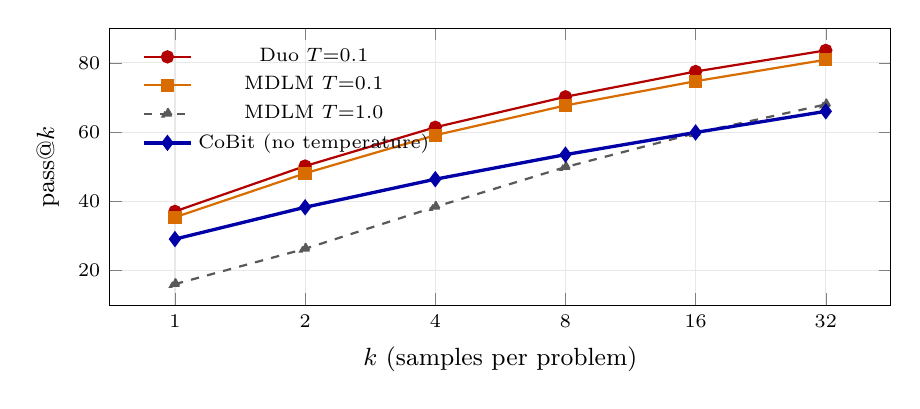
\begin{tikzpicture}
\begin{axis}[width=11.5cm,height=5.1cm,xmode=log,log basis x=2,
  xlabel={$k$ (samples per problem)},ylabel={pass@$k$},
  xtick={1,2,4,8,16,32},xticklabels={1,2,4,8,16,32},
  ymin=10,ymax=90,grid=both,grid style={gray!18},
  legend pos=north west,legend style={font=\scriptsize,draw=none,fill=none},
  label style={font=\small},tick label style={font=\scriptsize}]
\addplot[thick,mark=*,red!70!black] coordinates {(1,37.1)(2,50.2)(4,61.4)(8,70.2)(16,77.5)(32,83.6)};
\addlegendentry{Duo $T{=}0.1$}
\addplot[thick,mark=square*,orange!85!black] coordinates {(1,35.4)(2,48.1)(4,59.1)(8,67.7)(16,74.7)(32,80.9)};
\addlegendentry{MDLM $T{=}0.1$}
\addplot[thick,mark=triangle*,gray!70!black,dashed] coordinates {(1,16.1)(2,26.3)(4,38.4)(8,49.9)(16,59.7)(32,68.0)};
\addlegendentry{MDLM $T{=}1.0$}
\addplot[very thick,mark=diamond*,blue!65!black] coordinates {(1,29.1)(2,38.3)(4,46.4)(8,53.5)(16,59.9)(32,66.0)};
\addlegendentry{CoBit (no temperature)}
\end{axis}
\end{tikzpicture}
\end{center}

\vspace{-4pt}
{\large\bfseries What the numbers actually say}

\textbf{1. Low-$T$ does not cost headroom; it adds it.} MDLM $T{=}1.0\!\to\!0.1$ lifts pass@1
$16.1\!\to\!35.4\%$ \emph{and} pass@32 $68.0\!\to\!80.9\%$. Sharpening improves the ceiling that
post-training could realise, which is the opposite of the RLVR intuition
(Yue et al., \href{https://arxiv.org/abs/2504.13837}{arXiv:2504.13837}) we built the thesis on.

\textbf{2. The trade is real but only in relative terms.} The $k{=}1\!\to\!32$ multiplier falls
$4.2\times \to 2.3\times$ when MDLM is sharpened --- diversity \emph{is} being spent --- but the
absolute curve still rises everywhere. Relative climb is the wrong figure of merit.

\textbf{3. CoBit's own headroom is large but not competitive here.} $29.1\!\to\!66.0\%$
($2.3\times$) with $\mathrm{ESS}{=}32/32$, i.e.\ 32 genuinely independent churn samples,
no tempering and no selection. It remains the best \emph{continuous} model, and is best overall
on Sudoku, but on GSM8K tuned discrete diffusion dominates at every sampling budget --- not just
at $k{=}1$, as the COLM draft concedes.

\vspace{2pt}
{\large\bfseries Status and caveats}

Four of six cells are complete. \texttt{duo\_T1.0} crashed
(\texttt{OverflowError: int too large to convert to float} in their metrics path, not OOM) and
S-FLM has not run; both are needed to finish the temperature contrast.
Numbers are on 256 of 1319 problems ($\pm$3 points); the complementary 1063 are queued for CSD3
and merge by concatenation. pass@$k$ costs $k\times$ NFE, so these are \emph{headroom}
measurements, not matched-budget results. Reproduction note: our Duo $T{=}1$ single-sample is
19.5\% vs.\ 17.2\% published --- 95\% CIs overlap ([17.4,\,21.6] vs.\ [15.2,\,19.2]).

\vspace{2pt}
{\large\bfseries Implication for the workshop paper}

The ``diversity-vs-headroom'' framing is dead and should not be written. The defensible paper is
the \emph{evaluation} one: no prior work (S-FLM included --- one sample per problem, no pass@$k$
anywhere) reports multi-sample metrics on these benchmarks, and doing so overturns a natural
intuition about what low-temperature decoding costs. CoBit is the continuous entrant, strongest
on Sudoku; the GSM8K result is an honest negative that sharpens the existing concession.
\end{document}
